\documentclass[11pt]{book}
\usepackage[utf8]{inputenc}	% Para caracteres en español

\usepackage[left=2.75cm,right=2.75cm,top=2cm,bottom=3cm]{geometry}
\usepackage{style}



\begin{document}
\setcounter{section}{8}
\title{Algèbre linéaire I}
\maketitle
\thispagestyle{empty}

\begin{center}
\chapter{Calcul matriciel}
\begin{framedate}
    (10/10/2024)
\end{framedate}
\end{center}
\section{Déterminant et opération élémentaire}
\subsection{Application des opération élémentaire sur le déterminant}
\begin{itemize}
    \item Type I: Interchanger des lignes entre elle ne change pas le déterminant
    \item Type II: changer le signe de la matrice change le signe du déterminant
    \item Type III: En multipliant une ligne par un scalaire $\alpha \in \mathbb{R}$ , le déterminant est aussi multiplier par ce scalaire.

     
\end{itemize}

La preuve est par récurrence, le but est d'initialiser pour des matrice $M_{2\times 2}(\mathbb{R})$ et de le prouver pour des matrice de taille $n+1\times n+1$. 
\\
On suppose donc le résultat vrai pour les matrices de taille $\leq n$ et on passe au cas $M_{n+1\times n+1}(\mathbb{R})$. Ici $n \geq 2$. Comme une opération élémentaire fait intervenir au plus deux lignes, il existe une ligne $L_i$ qui ne change pas. On développe alors det(E*A) selon $L_i$ et on obtien la même formule que $det A$, où les * où $E$ est la matrice d'une opération élémentaire sous-déterminant, det $A_{ij}$ ont été remplacés par det E'$A_{ij}$ où E' est bien une matrice d'opération élémentaire équivalente à E.
\begin{framedremark}
    On écrit parfois $det A = |A|$.
\end{framedremark}
    

\begin{exemple}
Le détérminant  de:
\[\begin{vmatrix}
5 & 4 & 4 & 1\\
2 & 3 & 2 & -2 \\
-5 & -7 & -6 & 9 \\
1 & -2 & -2 & -4
\end{vmatrix}\]
\\
Le but est d'avoir que deux 0 sauf à une endroit sur la ligne 2:
\\
On peut par exemple faire $C_1 - C_3$ et $C_4 + C_3$, on a:
$\begin{vmatrix}
1 & 4 & 4 & 5\\
0 & 3 & 2 & 0 \\
1 & -7 & -6 & 3 \\
3 & -2 & -2 & 2
\end{vmatrix}$ $\to 2\cdot$ $\begin{vmatrix} 
1 & 4 & 2 & 5\\
0 & 3 & 1 & 0 \\
1 & -7 & -3 & 3 \\
3 & -2 & -1 & 2
\end{vmatrix}$
\\
On sort le facteur 2 de $C_3$ et donc il faut multiplier le det avec (Type III), On fait maintenant $C_2 3C_3$:

 \[2\cdot\begin{vmatrix} 
1 & -2 & 2 & 5\\
0 & 0 & 1 & 0 \\
1 & 2 & -3 & 3 \\
3 & 1 & -1 & 2
\end{vmatrix}\]

En utilisant les cofacteur on a que:
\[ det A = 2[-0\cdot detA_{21} + 0\cdot detA_{22} -1\cdot \begin{vmatrix} 
1 & -2 & 5\\
1 & 2  & 3 \\
3 & 1  & 2
\end{vmatrix}] = -2\cdot\begin{vmatrix} 
1 & -2 & 5\\
1 & 2  & 3 \\
3 & 1  & 2
\end{vmatrix}\]
On fait le même procédé ($L_2 - L_1$ et $L_3 - 3L_1$):
\[ -2\cdot\begin{vmatrix} 
1 & -2 & 5\\
1 & 2  & 3 \\
3 & 1  & 2
\end{vmatrix} \to -2\cdot\begin{vmatrix} 
1 & -2 & 5\\
0 & 4  & -2 \\
0 & 7  & -13
\end{vmatrix}\]
Ce qui nous donne à la fin:
\[ = -2\cdot 1 \cdot \begin{vmatrix}
    4 & -13 \\
    7 & -13
\end{vmatrix} = -2\cdot 1 [-52 + 14] = 76\]


\end{exemple}
\paragraph{Propriétés du déterminant}
\\

Soit $A$ une matrice de taille $n \times n$ et $\lambda \in \mathbb{R}$ Alors, $det (\lambda A) = \lambda^n \cdot det A $.
\begin{preuve}
    $\lambda \cdot A$ est obtenu de $A$ en effectuant $n$ opération élémentaires de type III (sur chacune des lignes).
    \end{preuve}
    \begin{framedremark}
        Si une ligne de $A$ est combinaison linéaire des autres lignes, alors $det A = 0$.
    \end{framedremark}
    \begin{theorem}
        Une matrice carrée est inversible si et seulement si det$A \neq 0$.
    \end{theorem}
    \begin{preuve}
        Une matrice carré est inversible $n\times n$ iff elle a $n$ pivots iff il existe des opérations élémentaires qui transforment A en une matrice échelonnée avec des pivots, non nuls, sur la diagonale.
        \\
        Le déterminant de cette matrice est le produit des termes de la diagonale, et il est non nul, donc $det A \neq 0$.
    \end{preuve}
    \begin{framedremark}
        Le déterminant a peut être changé de signe ou été multiplié par $\alpha \neq 0$, mais il reste $\neq 0$.
    \end{framedremark}
    
    \begin{theoreme}
        $det(A^t) = detA$
    \end{theoreme}
    \begin{preuve}
        Le développement du déterminant de $A$ selon la première ligne est identique au développement du déterminant de sa transposée selon la première colonne.
    \end{preuve}
    \begin{thm}
        Soit $A$ et $B$ deux matrices $n\times n$. Alors: 
        \\
        \[det(AB) = detA \cdot det B\]

    \end{thm}
    \begin{preuve}
        La preuve se fait en deux parties selon, selon que la matrice A est inversible ou non. 
        \begin{itemize}
            \item Supposons que $A$ soit inversible. Alors nous savons que $A$ peut s'écrire comme produit des matrices élémentaire. La preuve se fait par induction sur le nombre de matrices élémentaires.
            \item Pour initialiser l'induction on doit traiter le as où $A$ est une matrice élémentaire. Il y a donc trois sous-cas.

        \end{itemize}
    \end{preuve}
    \begin{enumerate}
        \item $A = E_{ij}(\lambda)$ est de type I. Comme elle est triangulaire et que sa fiagonale est constituée de 1, on a à $det(E_{ij}(\lambda) = 1$. Il faut encore calculer $det(E_{ij}(\lambda)B)$. \\ det
        \item $A = E_{ij}$, $det E_{ij} = -1$ car c'est $I_n$ avec $L_i$ et $L_j$ élanguées.
        \item $A = E_i(\lambda)$, $det(E_i(\lambda) = \lambda$ (diagonale. $det(E_i(\lambda)\cdot B) = \lambda \cdot detB = det E_{j}(\lambda)\cdot det B$.


    \end{enumerate}
    \textbf{Hypothèse de récurrence} : \[ det(AB) = det A \cdot det B\]
    Pour toutes les matrices $A$ qui sont produits d'au plus $n$ matrices élémentaires.
    \\
    \textbf{Pas de récurrence}. Considérons une matrice $A = E_{n+1} \cdot E_n ...$, qui est le produit de $n + 1$ matrices élémentaires. Nous devons montrer que:
    \[
    det(E_{n+1}\cdot E_n ... E_1 \cdot B) =  det(E_{n+1}\cdot E_n ... E_1)\cdot B    \]
    On sait que $det( E_n ... E_1) = C$ donc $det(E_{n+1}\cdot E_n ... E_1 \cdot B) = det(E_{n+1}) \cdot C$.
    On fait la suite jusqu'à trouver : \[
    det(E_{n+1}\cdot E_n ... E_1)\cdot B
    \]

    \paragraph{$2^{e}$ cas: } $A$ non inversible, Alors par le thèorème précédent, $det A = 0$. Donc $det(A) \cdot det(B) = 0$.\\
    On montre que $A\cdot B $ n'est pas inversible si bien que $det(A\cdot B) = 0$. Si $AB$ est inversible il existe $C$ tel que $(AB)C = I_n$ et $A(BC) = I_n$ mais on sait que $A$ n'est pas inversible, \textbf{Contradiction}.
    \\
    \paragraph{Corollaire} Si $A$ est inversible, alors \[det(A^{-1}) = \frac{1}{det A}\]
    \begin{framedremark}
        Même si en général $AB \neq BA$ on a toujours $det(AB) = (detBA)$ car les deux détérminants donnent $det A \cdot det B = det B \cdot det A$.
    \end{framedremark}
    \begin{framedremark}
        
    
        Attention : \[ det(A + B) \neq det A + det B\]
        Le déterminant n'est pas \textbf{linéaire} comme application, $det : M{n\times n} \to \mathbb{R}$.
    
    \end{framedremark}


    \paragraph{Linéarité du déterminant comme fonction \textbf{d'une colonne}}
    Le déterminant est linéaire comme fonction d'une colonne, pour cela nous devons vérifier:
    \begin{enumerate}
        \item $T(\vec{0}) = 0$ car c'est le déterminant d'une matrice ayant une colonne nulle.
        \item $T(\lambda\vec{x}) = \lambda T(\vec{x})$ car il s'agit d'une opération de type III sur la $j^{eme}$ colonne.
        \item $T(\vec{x}+ \vec{y}) = T(\vec{x}) + T(\vec{y})$ se prouve en développant le déterminant selon la $j^{eme}$ colonne.

    \end{enumerate}


    $A  \in M_{3\times3}(\mathbb{R})$, il faut alors tout développé mais faut juste le faire avec la commutativé et distributivité dans les nombres réels.

    \paragraph{Règles de Charmer}
    \begin{theoreme}
        
    
    Si $det A = ad-bc \neq 0$, le système
    \begin{align*}
        ax + by &= e\\
        cx + dy &= f
    \end{align*}
    A une solution unique (qu'on trouve grâce à la matrice inverse)
    \end{theoreme}
    \\
    
la solution du système est $A^{-1}\vec{b}$: 
\[\frac{1}{ad -bc}\begin{pmatrix}
    d & -b \\
    -c & a
\end{pmatrix}
\begin{pmatrix}
    e \\
    f
\end{pmatrix}\]
Alors : 
\[x = \frac{ed -bf}{ad -b} =  \frac{det\begin{pmatrix}
    e & b \\
    f & d
\end{pmatrix}} {det A}\]
Et:
\[
y = \frac{af - ec}{ad - bc} = \frac{det \begin{pmatrix}
    a & e \\
    c & f
\end{pmatrix}}{det A}
\]
Soit $A$ une matrice carrée \textbf{inversible}. Pour tout vecteur $\vec{b}$ on pose :
\[A_i\vec{b} = (\vec{a_1}... \vec{a}_{i-1} \vec{b} \vec{a}_{i+ 1} ... \vec{a}_n)\]

    La seul solution du système $A\vec{x} = \vec{b}$ est donnée par la formule : 
    \[
    x_i = \frac{detA_i(\vec{b})}{det A}
    \]
\subparagraph{Preuve.}
Soit $B_i = (I_n)_i(\vec{x}) = (\vec{e}_1,\dots, \vec{e}_{i-1}, .., \vec{e}_{i+1}, .., \vec{e}_n  $.
\\
La ligne $L_i$ est constituées de zéros, saut le coefficient $x_i$ en position $(i, i)$, si bien que $\det (B_i) = x_i$.
\\
$A$ étant inversible, la solution unique est:
\[\vec{a} = A^{-1}\vec{b}\]
\\
Soit $B_i = (I_n)_i(\vec{x}) = (\vec{e}_1,\dots, \vec{e}_{i-1}, .., \vec{e}_{i+1}, .., \vec{e}_n)$.
\\
\[\det B_i = x_i\]
On calcule:
\\
\begin{align*}
A\cdot B_i &= A\cdot(\vec{e}_1, ..., \vec{x}, ..., \vec{e}_n)\\
&= (A\cdot\vec{e}_1, ..., A\cdot\vec{x}, ..., A\vec{e}_n)\\
&= (\vec{a}_1, ..., \vec{b} .., \vec{a}_n)    
\end{align*}
\\
Ainsi \[\det(A_i(\vec{b})) = \det(A\cdot B_i) = \det A \cdot \det B_i\]
\\
En divisant par $\det A \neq 0$, on obtient notre formule:
    \[
    x_i = \frac{detA_i(\vec{b})}{det A}
    \]
\paragraph{La dimension rappel}
\lecture{13}{2024-10-29}{Base, noyau, image}{}
\begin{theoreme}
    Deux bases $V$ de ont le même nombre d'éléments
\end{theoreme}

\begin{definition}
    Soit $V$ un espace vectoriel et $\mathcal{B} = (e_1, \dots, e_n)$ une base. La \textcolor{red}{dimension} de $V$ est $n$. On note $dim V = n$.
\end{definition}
\begin{framedremark}
    On peut prendre par exemple les bases les plus connues:
    \begin{itemize}
        \item $dim $\R$^n = n$
        \item $dim \mathbb{P}_n = n + 1$
        \item $dim M_{m \times n}($\R$) = mn$
    \end{itemize}
\end{framedremark}

\begin{definition}
    Un espace vectoriel $V$ est de dimension nulle si et seulement si $V = \{0\}$.
\end{definition}
0 est un vecteur linéairement dépendant, il ne peut donc faire partie d'aucune base. La convention dite auparavant est : $Vect\{\emptyset\} = \{0\}$. Ainsi l'ensemble vide est une famille livre de générateur de $\{0\}$.

\begin{theoreme}[de la base incomplète]
    Soit $V$ un espace vectoriel de dimension $n$ et $\{e_1, \dots, e_k\}$ une famille libre de veteurs de $V$. Il exciste alors des vecteurs $e_{k+1}, \dots, e_n$ tels que ($e_1, \dots, e_n)$ forme un base de $V$.
\end{theoreme}
\begin{framedremark}
    Attention à ne pas confondre une base et des vecteurs c'est pour ça qu'ici on choisit des parenthèse pour une base et des allocalade pour une famille de vecteurs.
\end{framedremark}

\subparagraph{preuve} So $(e_1, \dots, e_k)$ forme déjà une base de $V$, on s'arrête là.\\
Sinon il existe un veteur $e_{k+1}$ qui n'est pas dans $Vect\{e_1, \dots, e_k\}$. J'affirme que $\{e_1, \dots, e_k, e_{k+1}\}$ est libre.
\\
\begin{itemize}
    \item En effet si $\alpha_1e_1, \cdots + \alpha_ke_k + \alpha_{k+1}e_{k+1} = 0$ alors $\alpha_{k+1} = 0$ car $e_{k+1}$ n'est pas combinaison linéaire des autres $e_j$ par construction.
    \item Ainsi $\alpha_1e_1 + \cdots + \alpha_ke_k  = 0$.
    \item Comme la famille de départ est libre, tous les $\alpha_i$ sont nuls
    \item On peut donc ajouter $e_{k+1}$ à la famille $\{e_1, \dots, e_k\}$
\end{itemize}
On continue ce processus inductif jusqu'à compter $n$ vecteurs


\begin{exemple}
Dans $M_{2 \times 3}(\mathbb{R})$, $dim = 6$ on prend les quatre matrices:
\[A = \begin{pmatrix}
    1 & 0 & 0 \\ 1 & 1 & 0
\end{pmatrix} ,  B = \begin{pmatrix}
    1 & 1 & 0 \\ 0 & 1 & 0
\end{pmatrix}, C  = \begin{pmatrix}
    1 & 0 & 0 \\ 0 & 1 & 0
\end{pmatrix}, D = \begin{pmatrix}
    1 & 0 & 0 \\ 0 & -1 & 0
\end{pmatrix}\]
Si on écrit ces matrices dans la base canonique de $M_{2\times 3}(\mathbb{R}), \mathcal{C}an$ et qu'on créer une matrice avec les lignes de ces vecteurs on a:
\[M = \begin{pmatrix}
    1 & 0 & 0 & 1 & 2 & 0\\
    1 & 1 & 0 & 0 & 1 & 0\\
    1 & 0 & 0 & 0 & 1 & 0 \\
    1 & 0 & 0 & 0 & - 1 & 0 \\
\end{pmatrix} \to \begin{pmatrix}
    1 & 0 & 0 & 0 & 1 & 0\\
    0 & 1 & 0 & 0 & 0 & 0\\
    0 & 0 & 0 & 1 & 0 & 0 \\
    0 & 0 & 0 & 0 & - 2 & 0 \\
\end{pmatrix} \]
On voit ici qu'il y a deux vecteurs be sibt oas des colonnes pivots ($e_{13}, e_{23})$, il ne sont donc pas combinaison linéaire de $A'$ ni de $A$.
\\
Et donc $(A, B, C, D, e_{13}, e_{23})$ est une base de $M_{2\times 3}(\mathbb{R})$.
\begin{framedremark}
    On a rajouter $e_{13}$ et $e_{23}$ car il ne sont pas combinaison linéaire.
\end{framedremark}
\end{exemple}

\paragraph{Deux points de vue sur les bases}
Soit $V$ un espace vetoriel de dimension $n$. Une \textcolor{red}{base} est une famille ordonnée de générateurs libre de $V$. Nous avons vu que toute base est composée du même nombre $n$ de vecteurs.
\\
\textbf{Critères}
\begin{itemize}
    \item Une famille libre $\mathcal{L}$ de $n$ vecteurs forem une base de $V$
    \item une famille génératrice $\mathcal{G}$ de $n$ vecteurs forme une base de $V$.
\end{itemize}
\\

Soit $\mathcal{F}  = \{f_1, \dots, f_k\}$ une famille génératrice de $V$ et $\mathcal{B} = (e_1, \dots, e_n)$ une base de $V$. Pour extraire une base de $\mathcal{F}:$
\begin{itemize}
    \item trouver les composantes des $f_j$ dans la base $\mathcal{B}$
    \item Ecrire la matrice $F$ dont les \textcolor{red}{colonnes} sont les $(f_j)_{\mathcal{B}}$.
    \item Echelonner $F$. (sur les lignes)
    \item Ne garder que les $n$ colonnes pivots de $F$.
    
\end{itemize}

\begin{exemple}
    Extraire de la famille $\{1 - t, -1 + t^2, t^2 - t, 1 + t, t^2 + 1\}$ une base de $\mathbb{P}^2$. On choisit la base canonique de $\mathbb{P}^2$:
    \[(1-t)_{\mathcal{C}an} = \begin{pmatrix}
        1 \\ -1 \\ 0
    \end{pmatrix}, (-1+t^2)_{\mathcal{C}an} = \begin{pmatrix}
        -1 \\ 0 \\ 1
    \end{pmatrix}, \dots \text{et on écrit:}\]
    \[A = \begin{pmatrix}
         1 &-1&0 & 1 & 1 \\
        -1&0&-1&1&0\\
         0&1&1&0&1
    \end{pmatrix} \to \begin{pmatrix}
         1 &-1&0 & 1 & 1 \\
        0&-1&-1&2&1\\
         0&0&0&2&2
    \end{pmatrix}\]
    La prochaine étape après avoir échelonner et de ne garder que les $n$ colonnes pivots de $F$, on voit donc choisir ici $3$ vecteurs qui ont chacun un pivot sur une ligne différente, les colonnes $1, 2, 4$. Ce qui donne:
    \[\mathcal{B} = (1-t, 1+t^2, 1+t)\] \textcolor{red}{Attention!}, on prend les colonnes qui sont les vecteurs et non directement les valeurs trouvées lorsqu'on échelonne. on prend les vecteurs qui se trouvaient sur les colonnes $1, 2, 4$.
\end{exemple}

\paragraph{Comment compléter une base}
Soit $\mathcal{F} = \{f_1, \dots, f_k\}$une famille libre de $V$ dont on a une base $(e_1, \dots, e_n)$. Pour compléter $\mathcal{F}$ en une base:
\begin{itemize}
    \item Trouver les composantes des $f_j$ dans la base $\mathcal{B}$.
    \item Ecrire la matrice $F$ dont les \textcolor{red}{lignes} sont les $(f_j)_{\mathcal{B}}$
    \item Echelonner $F$. (comme d'habitude)
    \item Ajouter les vecteurs $e_i$ pour les valeurs de $i$ qui ne son pas des colonnes pivot.
\end{itemize}

\begin{exemple}
    Compléter la famille $\{\vec{e_2} -\vec{e_1}, \vec{e_3} -\vec{e_1}, \vec{e_4} - \vec{e_1}\}$ en un base de \R$^4$.
    \[A = \begin{pmatrix}
        -1 & 1 & 0 & 0 \\
        -1&0&1 & 0\\
        -1&0&0 & 1
    \end{pmatrix}\to \begin{pmatrix}
        -1 & 0 & 0 & 1 \\
        0&1&0 & -1\\
        0&0&1 & -1
    \end{pmatrix} \]
    On voit qu'il y a pas de pivot sur la dernière colonne.
\end{exemple}


\paragraph{Rappels application linéaires:}
Soit $V$ et $W$ deux espaces vectoriels.
\begin{definition}[application linéaire]
    Une application $T : V \to W$ est \textcolor{red}{linéaire} si
    \begin{enumerate}
        \item $T(u + v) = Tu + Tv$ pour tous $u, v \in V$
        \item $T(\alpha v) = \alpha Tv$ pour tous $v \in V$ et $\alpha \in $\R
    \end{enumerate}
\end{definition}
\begin{exemple}
    \begin{enumerate}
        \item La dérivée $D : \mathcal{C}^\infty(\mathbb{R}) \to \mathcal{C}^\infty(\mathbb{R}) $ des a faire plus tard
    \end{enumerate}

    Contre exemple:
    \\ 
    L'application $C : \mathbb{P}_2 \to \mathbb{P_4}$ définie par 
    \begin{formule}
\begin{center}
    $p \to p^2$
    \end{center}

    \end{formule}
    n'est pas linéaire. En effet on voit par exemple que:
    \[C(2t) = (2t)^2 = 4t^2 \neq 2t^2 = 2C(t)\]
    \begin{framedremark}
        Généralement, les applications linéaires n'aiment pas quand on les met au carrées.
    \end{framedremark}
\end{exemple}


\paragraph{Noyau}
Soit $T: V \to W$ une application linéaire.
\begin{definition}
    Le \textcolor{red}{noyau} de $T$ est le sous-ensemble $Ker T = \{v \in V | Tv = 0\}$.
\end{definition}
Ce qui veut dire que le noyau est le sous-ensemble des vecteurs qui ont pour image le zéro. donc si on prend par exemple les dérivées, on voit que tout les constantes ont la même image qui est 0 donc le noyaux de l'application linéaire des dérivées et le vecteur des constantes.
\begin{exemple}
    Soit $T: \mathbb{R}^2 \to \mathbb{R}^2$ la projection orthogonale sur l'axe $x = y$.
    On voit que c'est la droite $x$ on a donc que:
    \[T(\vec{e_1}) = \begin{pmatrix}
        \frac{1}{2}\\ \frac{1}{2}
    \end{pmatrix}, T(\vec{e_2}) = \begin{pmatrix}
        \frac{1}{2}\\ \frac{1}{2}
    \end{pmatrix}\]
La matrice de T est donnée par:
\[A = \begin{pmatrix}
    \frac{1}{2} & \frac{1}{2} \\
    \frac{1}{2} & \frac{1}{2}
\end{pmatrix}\]
Essayons de trouver le noyau:
\[A\cdot\begin{pmatrix}
    x \\ y
\end{pmatrix} = \begin{pmatrix}
    0 \\ 0
\end{pmatrix}\]
    On a donc fini avec deux équation qui sont:
    \begin{align*}
        \frac{1}{2}x + \frac{1}{2}y  &= 0\\
        \frac{1}{2}x + \frac{1}{2}y &= 0
    \end{align*}
    On peut déjà deviner ici que le noyau ne sera pas l'ensemble vide, on a deux équations identiques (donc une seule) avec deux variables, cela veut dire qu'il restera donc une variable libre:
    \begin{align*}
        y &= y \\
        y &= -x
    \end{align*}
    Ce qui donne : 
    \[Ker T = Vect\begin{pmatrix}
        -1 \\ 1
    \end{pmatrix}\]
    Ce qui si on le voit graphiquement est assez intuitif:
    Prenons la droite $y = -x$ et $y = x$ on a:
\begin{center}
    

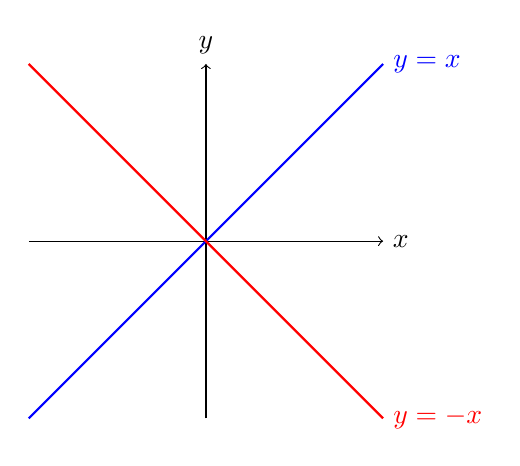
\begin{tikzpicture}[scale=0.75]
    % Axes
    \draw[->] (-3,0) -- (3,0) node[right] {\(x\)};
    \draw[->] (0,-3) -- (0,3) node[above] {\(y\)};

    % Droite y = x
    \draw[blue, thick] (-3,-3) -- (3,3) node[right] {\(y = x\)};

    % Droite y = -x
    \draw[red, thick] (-3,3) -- (3,-3) node[right] {\(y = -x\)};
    
\end{tikzpicture}
\end{center}
On voit que sur chaque point de la droite rouge, si on les ramènes sur la droite bleu (en faisant la projection) il arrive au point $(0, 0)$.
\end{exemple}








\begin{formule
} Cours 14 30/10/2024
\end{formule
}
\paragraph{Le noyau est un sous-espace}
\begin{exemple}
Soit $T : M_{2\times 2}($\R) $\to \mathbb{R}^2$ défini par:
\[T\begin{pmatrix}
    a & b \\ c & d
\end{pmatrix} = \begin{pmatrix}
    c \\ a-d
\end{pmatrix} = \begin{pmatrix}
    0 \\ 0
\end{pmatrix}\]
On vérifie que $T$ est linéaire. Le noyau de $T$ est un sous-ensemble de $M_{2\times 2}($\R). Lequel? C'est le sous-espace:
\[Ker T = \{ \begin{pmatrix}
    a & b \\ 0 & a
\end{pmatrix}|a, b \in \mathbb{R}\}\]
\end{exemple}

\begin{theoreme}
    Soit $T: V \to W$ une application linéaire. Alors $KerT$ est un sous-espace de $V$.
\end{theoreme}

\paragraph{Preuve}
\begin{enumerate}
    \item $0 \in Ker T$ : $T(0) = 0$ car $T$ est linéaire
    \item stabilité de $+$: Si $v, v' \in KerT$, on montre que $v+v' \in KerT$, ce qui donne $0 + 0 = 0$ (les images des éléments du noyau sont tous égaux à 0).
    \item Stabilité de l'action: comme c'est une application linéaire on peut surtout $\alpha$ de l'application, on a donc, $\alpha \cdot 0 = 0$.
\end{enumerate}


\begin{definition}
Soit $T : V \to W$ une application linéaire. Alors $T$ est injective si et seulement si $\ker T = \{0\}$ 
\end{definition}

\begin{exemple}
    On considère $T : \mathbb{R}^4 \to \mathbb{R}^2$ donné par
    \[A = \begin{pmatrix}
        1 & -1 & 1 & -1 \\ 1 & 1 & 1 & 1
    \end{pmatrix}\]
    On a donc que 
    \[Ker T = Ker A = \{\vec{v}\in \mathbb{R}^4| A \cdot \vec{v}= \vec{0}\}\]
    est la solution générale S du système homogène donné par $A$. Si on échelonne la matrice on obtient:
    \[\begin{pmatrix}
        1 & -1 & 0 & 0 \\ 0 & 0 & 1 & -1
    \end{pmatrix}\]
    On en vient à :
    \[S = Ker A = Vect \{ \begin{pmatrix}
        1 \\ 1 \\ 0 \\ 0
    \end{pmatrix}, \begin{pmatrix}
        0 \\ 0 \\ 1 \\ 1
    \end{pmatrix}\}\]
    Les deux vecteurs ici forment une base de $Ker A$.
    \\
    Juste pour expliquer comme on passe de la matrice à vect, on peut par exemple remettre en système d'équation classique du genre:
    \begin{align*}
        x -y + 0 + 0 &= 0\\
        0 + 0 + z - w &= 0
    \end{align*}
    On voit qu'il y aura deux variables libres, et donc:
    \begin{align*}
        x &= x \\
        y &= x\\
        z &= z\\
        w &= z
    \end{align*}
    Voila d'où vient les deux vecteurs, un en fonction de $x$ et l'autre en fonction de $z$.
\end{exemple}

\begin{definition}
    L'\textcolor{red}{image} d'une application linéaire $T : V \to W$ est le sous-ensemble $Im T = \{w \in W| \text{il existe } v \in V $ tel que $Tv = w\}$
\end{definition}
\begin{framedremark}
    Le concept d'image généralise la notion du sous-espace $Col A$ engendré par les colonnes d'une matrice A.
\end{framedremark}

\begin{theoreme}
    Soit $T : V \to W$ une application linéaire. Alors $Im T$ est un sous espace de $W$.
\end{theoreme}
\paragraph{Preuve}
On voit d'abord que $0 = T(0)$ appartient à l'image. Il reste à montrer la stabilité de la somme et de l'action. Traitons le cas de la somme. Soient donc $w, w'$ deux vecteurs de $Im T$. Nous devons montrer que $w + w'$ aussi appartient à $Im T$.
\\
On sait que $w, w' \in ImT$, donc il existe $v, v' \in V \text{tq} T(v) = w $ et $T(v') = w'$.\\
On choisit $v_2 = v + v'$ et on calcule par linéarité de $T$ : \[T(v_2) = T(v + v') = T(v) + T(v') = w + w'\]
Donc, $w + w' \in Im T$  (on a le droit de faire tout ça parce que $T$ est une application linéaire.
\\
Pour ce qui est de l'action, on peut juste faire le même procédé et grâce au faite que $T$ est une application linéaire, ça marchera aussi.


\begin{framedremark}
    Soit $T : V \to W$ une application linéaire. Alors $Ker T$ est un sous-espace de $V$, mais $Im T$ est un sous-espace de $W$. (Attention à où vit ces ensembles)
\end{framedremark}

\begin{exemple}
    Soit $D : \mathbb{P}_3 \to \mathbb{P}_3$ la dérivation, $D(p) = p'$.
    \begin{itemize}
        \item $Ker D = \{p \in \mathbb{P}_3 | p' = 0\} = \{a \in \mathbb{P}_3 | a \in $ \R $\}$ (le polynôme constants \[= Vect\{1\}\]

        \item $Im D = \{q \in \mathbb{P}_3 | \exists p \in \mathbb{P}_3$ avec $D(p)  = q\}$
\[= Vect\{1, t, t^2\} \subset \mathbb{P}_3\]
Pour expliquer un peu, on sait que tout les polynômes qui ont que des constantes vont sur $0$ donc on prend le vecteur des constantes qui lui nous ramène de toutes les constantes à $0$.\\
De l'autre côté, l'image reprends tout ce qui arrive de l'autre côté, on voit qu'il y a pas $t^3$ dans l'image, quand on dérive un polynôme, il devient de degrés $2$. Donc la base de l'image va, "\textit{avec le noyau}" et $t^2$

    \end{itemize}
\end{exemple}

\paragraph{Méthode de calcul}
Soit $T : \mathbb{R}^n \to \mathbb{R}^m$ une application linéaire, représentée par une matrice $A \in M_{m\times n}(\mathbb{R})$.
\begin{itemize}
    \item Pour calculer le \textcolor{red}{noyau} de $T$ on échelonne et réduit la matrice $A$ selon les \textcolor{red}{lignes}.
    \item Pour calculer l'\textcolor{blue}{image} de $T$ on ne garde que les \textcolor{blue}{colonnes-pivotss}. Si nécessaire on échelonne et réduit $A$ selon les \textcolor{blue}{colonnes}.
\end{itemize}

\begin{framedremark}{espace-colonne}
    On appelle parfois \textcolor{red}{espace-colonne} le sous-espcae $ColA$ engendré par les colonnes de $A$. Il s'agit donc de $Im A$
\end{framedremark}
\paragraph{explication de pourquoi ça marche}
Soit $A \in M_{m\times n}(\mathbb{R})$ et $B$ la matrice échelonnée associée ($B$ est juste la matrice échelonnée).
\\
SI une colonne n'a pas de pivot, le système $A\vec{x} = \vec{0} $ a une infinitén de solutions (les mêmes que $B\vec{x} = \vec{0}$), on peut écrire
\[x_1\vec{a}_1 + \dots + x_n\vec{a}_n = \vec{0}\]


\begin{framedremark}
    Les colonnes sans pivot sont combinaison linéaire des autres colonnes.\\ Les colonnes de $A$ vérifient les mêmes relations de dépendance linéaire que celles de $B$
\end{framedremark}
On peut donc enlever une telle colonne pour engendrer $ColA = ImA$. Les k colonnes-pivot restantes de $A$ sont libres puisque la matrice $m\times k$ formée de ces k colonnes a $k$ pivots.

\begin{exemple}
    On donnt une application linéaire donnée par $A$ tel que:
    \[A = \begin{pmatrix}
        1 & 0 & 0 & -1\\
        -1 & 1 & 0 & 0\\
        0 & -1 & 1 & 0 \\
        0 & 0 & -1 & 1
    \end{pmatrix} \to \begin{pmatrix}
         1 & 0 & 0 & -1\\
        0 & 1 & 0 & -1\\
        0 & 0 & 1 & -1 \\
        0 & 0 & 0 & 0
    \end{pmatrix}\]
    On voit qu'il y a une colonne sans pivot, donc le noyau a qu'une seule variable libre et donc comme on l'avait fait auparavant, on fixe le dernier l'élément, et on voit aussi que chaque $x_1, x_2, x_3$ sont égaux à $1$ ($1 -1  = 0 \to 1 = 1)$ on trouve que:
    \[Ker A = Vect\{\begin{pmatrix}
        1 \\ 1 \\1 \\1 \\
    \end{pmatrix}\}\]
    
\end{exemple}

\paragraph{Rappel critère d'injéctivité (encore)}
Le critère d'injectivité d'une application linéaire permet de ramener la démonstration de l'injectivité au calcul du noyau. Le noyau mesure donc le \textcolor{red}{défaut d'injectivité}.
\begin{theoreme}
    Une application linéaire $T: V \to W$ est injective si et seulement si $Ker T = \{0\}$ 
\end{theoreme}
\paragraph{Espaces-lignes: $LgnA$}
Soit $A$ et $B$ deux matrices de taille $m\times n$ On note $A  \textasciitilde B$ quand elles sont équivalentes selon les lignes.
\begin{theoreme}
    Si $A \textasciitilde B$ alors les lignes de $A$ et $B$ engendrent le même sous-espace de $\mathbb{R}^n$.   
\end{theoreme}
\textbf{Pourquoi?} Les opération élémentaires produisent de nouvelles lignes qui sont cominaison linéaires des précédentes.
\begin{theoreme}
    Les lignes d'une forme échelonnée de $A$ forment une base du sous-espace engendré par les lignes de $A$.
\end{theoreme}
\textbf{Pourquoi?} Aucune ligne non nulle de la forme échelonnée ne peut être combinaison linéaire des autres (à cause de son pivot)

\paragraph{Espaces-colonnes: $ColA$}
Soit $A$ une matrice de taille $m \times n$.
\begin{theoreme}
    Les colonnes pivots de $A$ forment une base de $ColA = Im A$.
\end{theoreme}

\lecture{15}{2024-05-11}{Théroème du rang}{}
\begin{parag}
    

\begin{subparag}{remarque importante}
Soit $A$ une matrice de taille $m \times n$.
\begin{theoreme}

    $dim ColA = dim\; LgnA$

\end{theoreme}
\begin{itemize}
    \item Le nombre de lignes linéairement indépendantes est égal au nombre de lignes contenant un pivot.
    \item Le nombre de colonnes linéairement indépendantes est égal au nombre de colonnes contenant un pivot.
    \item En résumé, $dim\; ColA = dim\; LgnA$ car les deux dimensions coïncident avec le nombre de pivots.

\end{itemize}
    
\end{subparag}


\begin{subparag}{exemple}

Le cas d'une matrice $2\times 2$.
Soit $A =  \begin{pmatrix}
    0 & 0 \\ 0 & 0
\end{pmatrix}$, alors $dim\; LgnA = 0 = dim \; ColA$.\\
Supposons que $A \neq 0$, alors $A = \begin{pmatrix}
    a & b \\ c & d
\end{pmatrix}$. Si les deux colonnes sont proportionelles, $dim\; ColA = 1$  On peut supposer que $\begin{pmatrix}
    b \\ d
\end{pmatrix} = \begin{pmatrix}
    \lambda a \\ \lambda c
\end{pmatrix}$ pour une $\lambda \in $\R. 
\[A = \begin{pmatrix}
    a & \lambda a \\ c & \lambda c
\end{pmatrix}\]
\textbf{Premier cas:} $a = 0$, aussi $\lambda a = 0$ et comme $A \neq 0$, $dim \; LgnA = 1$ ca la $2^e$ ligne est non nulle.
\\
\textbf{deuxième cas} $a \neq 0$ $\begin{pmatrix}
    a & \lambda a \\ c & \lambda c
\end{pmatrix}  $ a deux lignes proportionnelles car $\left(c \; \lambda c\right) = \frac{c}{a}\left(a \; \lambda a\right)$. Ici aussi $dim \; LgnA = 1$.
    
\end{subparag}

\end{parag}

\begin{parag}{Le Théorème du rang}
    



\paragraph{A faire plus tard parce que je sais pas}
    On se ramène au cas d'une application linéaire $R^n \to R^m$, représentée par $A \in M_{m\times n}\left(\mathbb{R} \right)$.
    \begin{enumerate}
        \item On choisit une base $\mathcal{B} = \left(e_1, \dots, e_n\right)$ de $V$
        \item On considère la composition suivante
 \item     \end{enumerate}


\begin{theoreme}{théorème du rang}
    
        \[rangT + dim\; KerT  = dimV\]
    
\end{theoreme}
\begin{itemize}
    \item Grâce aux coordonnées on identifire $V$ avec \R$^n$ et W avec \R$^m$.
    \item Ainsi on identifire $T$ avec une application linéaire $S: \mathbb{n} \to \mathbb{R}^m$.
    \item Celle-ci est donnée par la multiplication matricielle \[\vec{x} \to A\vec{x} = S\left(\vec{x}\right)\]
    \item $dim \; KerA = $ nombre de colonnes sans pivot
    \item $dim \; ImA = \text{rang}A = $ nombre de colonnes-pivot
    \item  nombre de colonnes-pivot $+$ colonnes sans pivot $= n$.
\end{itemize}

\begin{subparag}{Idée de la preuve}
    

Si $dim V = n$, $dim \; KerT = k \leq n$ car $KerT \subset V$. On choisit une base $\left(e_1, \dots, e_k\right)$ de $KerT$. Grâce au Théorème de la base complétée, il existe $\left(e_{k+1}, \dots, e_n\right)$  tel que $\left(e_1, \dots, e_k, e_{k+1}, \dots, e_n\right) $ est une base de V. 
\\
Alors $\{T\left(e_1\right), \dots, T\left(e_k\right), T\left(e_{k+1}\right), \dots, T\left(e_n\right)\}$ engendrent $ImT$.
\\
Donc $\{T\left(e_{k+1}, \dots, T\left(e_n\right)\right)\}$ engendrent $ImT$.
\\
Mais T | $Vect\{e_{k+1}, \dots, e_n\}$ est injective car $KerT \cap U = \{0\}$.
Donc $T\left(e_{k+1}\right), \dots, T\left(e_n\right)$ sont libres, donc forment une base. Conclusion \[RangT  = n - k\]
\end{subparag}


\begin{definition}
Soit $T : V \to W$ une application linéaire entre espaces vectoriels de dimension finies.
\\
Le \textcolor{red}{rang} de $T$ est la dimension de l'image de $T$ : 
\[rang T = dim \; ImT\]
\end{definition}

\begin{definition}
Soit $A$ une matrice $m \times n$, représentant une application linéaire.
\\
    Le \textcolor{red}{rang} de $A$ est la dimension de l0image de $A: $ $rangA = dim\; ImA$.
\end{definition}
\begin{theoreme}{théorème du rang}
    
        \[rangT + dim\; KerT  = dimV\]
    
\end{theoreme}
    \begin{subparag}{Exemple}
        Considérons l'application linéaire $T: \mathbb{P}_2 \to $ \R$^2$ définie par:
        \[T\left(p\right) = \begin{pmatrix}
            p\left(0\right) \\ p\left(1\right)
        \end{pmatrix}\]
        Pour tout polynôme $p$ de degrès $\leq 2$.
        \\
        Nous allons 
        \begin{itemize}
            \item Calculer le noyau
            \item en déduire la dimension de l'image grâce au théorème du rang, et
            \item interpréter ce résultat pour conclure que deux zéros d'une fonction polynomiale de degrès $\leq 2$ déterminent le polynôme en question à un facteur près.
        \end{itemize}

        \begin{align*}
        Ker T &= \{p \in \mathbb{P}_2 | p\left(0\right) = 0 = p\left(1\right)\}\\
            &= \{p \in \mathbb{P}_2 | p\left(t\right) = a\cdot t\cdot \left(t - 1\right) \text{ , pour un } a \in \mathbb{R}\} \\
            &= Vect\{\left(t-1\right)\} \text{ de dimension 1.}
        \end{align*}
        Par le théorème du rang, $rang T + dim\;KerT = 3$ donc $rang T = 2 = dim \mathbb{R}^2$.
        \\
        L'interprétation suit: si $p\left(t\right)$ s'annule en $0$ et en $1$, alors $p\left(t\right) = a \cdot t \cdot \left(t- 1\right)$ pour $a \in $ \R.
    \end{subparag}
\end{parag}
 \begin{parag}{Critère d'inversibilité}
     Soit $A$ une matrice carrée de taille $n\times n $. Alors les conditions suivantes sont équivalentes : 
     \begin{enumerate}
         \item La matrice $A$ est inversible
         \item les colonnes de $A$ forment une base de $\mathbb{R}^n$.
         \item $ImA = \mathbb{R}^n$ \hspace{5cm} $A$ est surjective
         \item $dim \; Im A = n$.
         \item $rang\; A = n$
         \item $Ker\;A = \{0\}$ \hspace{4.75cm} $A$ est injective
         \item $dim\; Ker\; A = 0$.
     \end{enumerate}
     \begin{subparag}{Exemple}
         Pour quelles valeurs du paramètre réel $a$ la matrice $A$ suivante est-elle inversible?
         \[\begin{pmatrix}
             a & 1 & 1 & 1\\
             1 & a & 1 & 1\\
             1 & 1 & a & 1\\
             1 & 1 & 1 & a
         \end{pmatrix} \to \begin{pmatrix}
            1 & 1 & 1 & a\\
             0 & a-1 & 0 & 1-a\\
             0 & 0 & a-1 & 1-a\\
             0 & 1-a & 1-a & 1-a^
             
         \end{pmatrix}\]
         (les opérations sont $L_1 - L-4$, $L-2 - L_1'$, $L_3  L_1'$, $L_4 - a\cdot L_1'$)
         Si $a - 1 = 0$ alors $a = 1$ donc:
         \\
         $rang\; A = 1$, $dim \; Ker A = 3$
         \\
         Si $a \neq 1$, on peut diviser chaque ligne par $a-1$, on obtient alors:
 \[\begin{pmatrix}
            1 & 1 & 1 & a\\
             0 & 1 & 0 & -1\\
             0 & 0 & a-1 & -1\\
             0 & 1 & 1 & 1 + a
             
         \end{pmatrix} \to \begin{pmatrix}
            1 & 1 & 1 & a\\
             0 & 1 & 0 & -1\\
             0 & 0 & 1 & -1\\
             0 & 0 & 0 & a + 3
             
         \end{pmatrix}\]
         Les opération ici pour passer à la deuxième matrice sont ($L_3 - L_2 - L_3$) + $+$
     \end{subparag}
 \end{parag}

 \begin{parag}{Une application linéaire}
     Soit $W$ le sous-espace vectoriel de $M_{2\times2}\left(\mathbb{R}\right)$ des matrices triangulaires supérieures.
     \\
     En fait $W = Vect\{e_{11}, e_{12}, e_{22}$ et $\mathcal{B} = (e_{11}, e_{12}, e_{22})$ est une base de $W$.
     \\
     On considère $T : \mathbb{P}_2 \to W$ l'application linéaire définie par
     \[T\left(p\right) = \begin{pmatrix}
         p\left(1\right) & p\left(-1\right) \\
         0 & p\left(2\right)
     \end{pmatrix}\]
     En choisissant la base canonique $\mathcal{C}an = \left(1, t, t^2\right)$, on identifie $\mathbb{P}_2$ avec \R$^3$ et en choisissant la base ci-dessus de $W$ on identifie $W$ avec \R$^3$ également. Ce qui nous donne:
     \[\begin{pmatrix}
         1 \\ 0 \\ 0
     \end{pmatrix} = \vec{e}_1 = \left(1\right)_{\mathcal{C}an} \text{et} 1 \to \begin{pmatrix}
         1 & 1 \\ 0 & 1
     \end{pmatrix} = W_1 \text{et} \left(W_1\right)_{\mathcal{B}} = \begin{pmatrix}
         1 \\ 1 \\ 1
     \end{pmatrix}\]
     \[\begin{pmatrix}
         0 \\ 1 \\ 0
     \end{pmatrix} = \vec{e}_2 = \left(t\right)_{\mathcal{C}an} \text{et} t \to \begin{pmatrix}
         1 & -1 \\ 0 & 2
     \end{pmatrix} = W_1 \text{et} \left(W_2\right)_{\mathcal{B}} = \begin{pmatrix}
         1 \\ -1 \\ 2
     \end{pmatrix}\]
     \[\begin{pmatrix}
         0 \\ 0 \\ 1
     \end{pmatrix} = \vec{e}_3 = \left(t^2\right)_{\mathcal{C}an} \text{et} t^2 \to \begin{pmatrix}
         1 & 1 \\ 0 & 4
     \end{pmatrix} = W_3 \text{et} \left(W_3\right)_{\mathcal{B}} = \begin{pmatrix}
         1 \\ 1 \\ 4
     \end{pmatrix}\]
     \begin{subparag}{remarque}
         En gros on n'a juste "\textit{skip}" $a_{21}$ parce qu'il valait tout le temps $0$. Mais On aurait pu dire que l'ensemble $W$ est un sous-ensemble de $\mathbb{R}^4$ tel que $W \subset \mathbb{R}^4$.
     \end{subparag}
 \end{parag}

 \begin{parag}{Résumé}
     Le théroème du rang peut nous permettre de faire de grand raccourci lors de choix multiple.
     \begin{itemize}
         \item Le rang d'une matrice $A$ de taille $n \times m$ ne peut pas dépasser $n$.
         \[Rang  A + dim\; KerA = n\]
         \item Pour rappel, si on prend une application $A :$ $V \to W$ on a que $Ker A$ est dans $V$ et que $Im A$ est dans $W$.                               
     \end{itemize}
 \end{parag}

\end{document} 
